\documentclass[10pt,bibliography=totocnumbered,listof=totocnumbered, footsepline, headsepline]{scrreprt}
\usepackage[a4paper,top=2.5cm,left=2.5cm,bottom=2cm,right=2cm]{geometry}
\usepackage[english]{babel}
\usepackage[utf8]{inputenc}
\usepackage{amsmath}
\usepackage{mathtools}
\usepackage{amsfonts}
\usepackage{amssymb}
\usepackage{amstext}
\usepackage{graphicx}
\usepackage{tabularx}
\usepackage{setspace}
\usepackage[right]{eurosym}
\usepackage{subfig}
\usepackage[usenames,dvipsnames]{color}
\usepackage{colortbl}
\usepackage{array}
\usepackage{parskip}
\usepackage[right]{eurosym}
\usepackage[pdfpagelabels=true]{hyperref}
\usepackage{listings}
\usepackage[automark]{scrlayer-scrpage}
\usepackage{multicol}
\usepackage{float}
\usepackage{enumerate}
\usepackage{pgfplots}
\usepackage{xcolor}
\usepackage{todonotes}
\usepackage{fontawesome}
\usepackage{pdfpages}

\lstset{ %
	backgroundcolor=\color{white},   % choose the background color
	basicstyle=\footnotesize,        % size of fonts used for the code
	breaklines=true,                 % automatic line breaking only at whitespace
	captionpos=b,                    % sets the caption-position to bottom
	commentstyle=\color{ForestGreen},    % comment style
	escapeinside={\%*}{*)},          % if you want to add LaTeX within your code
	keywordstyle=\color{blue},       % keyword style
	stringstyle=\color{BurntOrange},     % string literal style
}

\definecolor{codegreen}{rgb}{0,0.6,0}
\lstdefinestyle{mystyle}{
    backgroundcolor=\color{black},
    basicstyle=\ttfamily\footnotesize\color{codegreen},
}

% Header Footer
\pagestyle{scrheadings}
\automark[section]{chapter}
\clearscrheadfoot
\ihead[]{TDDI08 and TDTS07 - Embedded Systems Design}
\ohead[]{Formal Verification with UPPAAL}
\ifoot[]{Simon Burkhardt (simbu448), Jule Enninghorst (julen905)}
\ofoot[]{\thepage}
\addtolength{\footskip}{-4ex}
% Section Deapth
\setcounter{secnumdepth}{4}

%\setcounter{section}{2}
\renewcommand{\thesection}{Assignment \arabic{section}:}
\renewcommand\thefigure{\arabic{figure}}

\renewcommand{\arraystretch}{1.2}


\begin{document}

\title{TDTS07/TDDI08 lab 2 - UPPAAL}
\author{Simon Burkhardt (simbu448)\\ Jule Eninghorst (julen905)}
\maketitle

\section{Getting Started}

The purpose of this task is to get familiar with the UPPAAL language syntax and expressions.

\url{https://docs.uppaal.org/language-reference/requirements-specification/}

\url{https://docs.uppaal.org/language-reference/requirements-specification/symb\_queries/}

\paragraph{Explanation of the template:} The following expression "\texttt{E<> P.s3}" of the UPPAAL "requirements specification language" uses the "\texttt{E<> p}" (Possibly) symbolic expression. In this case it asks if there is ever a sequence of states that reaches \texttt{P.s3}. In the state machine, there are three possible paths for this. a) $s0 \rightarrow s2 \rightarrow s3$ or b) $s0\rightarrow s1 \rightarrow s3$ or c) $s0 \rightarrow s1 \rightarrow s2 \rightarrow s3$. This first expression therefore evaluates to \texttt{true}.

The second expression "\texttt{A<> P.s3}" asks that all possible paths must \textbf{eventually} end in $s3$. The previous expression only asked for the possibility. This second expression asks for certainty. This is not given in our state machine, because there is no external trigger that forces states to change. So for example, the state machine could just loop in s0 forever. The expression therefore evaluates to \texttt{false}.

\section{Fischer 1}

This task compares the execution time of the same constraint verification runs for different system complexities. All time measurements were taken by hand using an Android smartphone. The uncertainty of the measurements is assumed to be within $\pm1$ s.

Finally, the task description asks for an estimation (not a measurement) of the Fischer system with $n=12$ independent participating processes.
According to the extrapolation using an exponential curve fit in Fig. \ref{fig:fisher_2_plot} it would take approximately $100$ s to verify the Mutex condition.

% \texttt{A[]} not deadlock = every reachable state satisfies "not deadlock"

\begin{figure}[H]
	\centerline{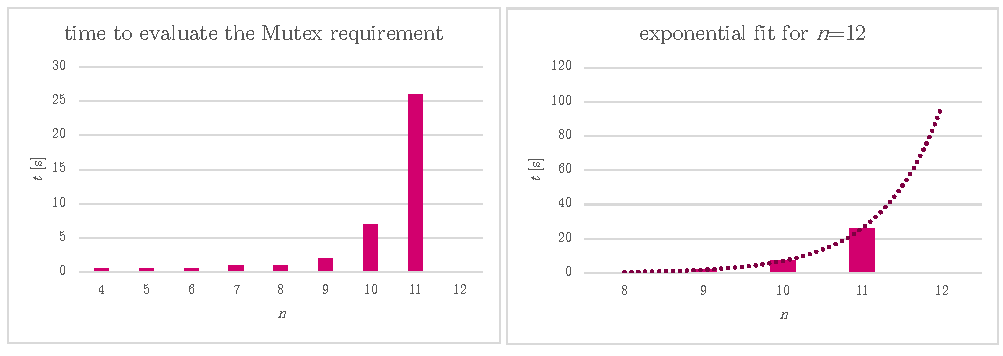
\includegraphics[width=38pc]{fischer_2_plot.pdf}}
	\caption{Time measurements to validate different sizes $n$ of the system}
	\label{fig:fisher_2_plot}
\end{figure}

\textbf{System Info}\\

CPU: Intel Core i5-2400 (64 Bit) @ 3.10 GHz running Centos-7



\section{Fischer 2}

If $m<k$ the Mutex requirement will not be satisfied.
Fig. \ref{fig:Fisher_2_violation_trace} gives an example for a sequence of state transitions that results in such an invalid state.

However, under the condition $m \geq k$, the Mutex requirement is also satisfied.

\begin{figure}[H]
	\centerline{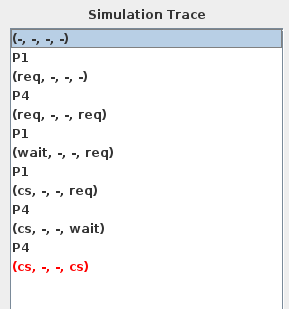
\includegraphics[width=12pc]{Fisher_2_violation_trace.png}}
	\caption{One of many possible traces that violate the constraint that no more than one P can be in state cs.}
	\label{fig:Fisher_2_violation_trace}
\end{figure}

\section{Traffic Light Controller}

The traffic light controller is implemented using three templates. Two for the respective axes (NS and EW) and one for the timer. We chose to have two templates for the two axes as they have to listen to opposite channels in order to be granted a green light. Otherwise, the two templates function the same way.\\
The timer is simply sending a signal on the channels \texttt{enableNS} and \texttt{enableWE} alternating every 5 seconds as defined by the \texttt{TIMEOUT} variable. This allows for a constant change of enabled axis to let cars drive from the NS-direction as well as from the WE-direction.\\
A process for a traffic light starts in the initial state of \texttt{RED} representing the fact that the light is currently red and no cars are waiting. Should a car arrive at this traffic light a boolean vairable \texttt{car} is set to true (we only are interested \textit{if} a car is waiting not how many cars are waiting) and the state changes to \texttt{WAIT} (i.e., the light is still red but now cars are waiting for the light to turn green). In the \texttt{WAIT} state the process is listening to the signal \texttt{enableNS} if on the NS-axis or \texttt{enableWE} if the light is on the WE-axis. When a signal is received (i.e., the traffic light process is synchronized with the timer) it changes to the state \texttt{GREEN}, representing that the waiting car is given a green light. It stays in that state for as long as the perpendicular axis does not get enabled. When changing back to the \texttt{RED} state, the boolean variable of a car waiting is set to \texttt{false}. Back in the \texttt{RED} state the circle continues again.\\
We created two process instances of each template representing the N and S direction as well as the E and W direction. In the verifier we check that the system does not deadlock and that each process can eventually end up in a green light for their cars. Moreover, we ensured the important safety constraint which states that the lights on the perpendicular axes cannot be simultaneously green. And last but not least, we check the constraint that if a car arrives on a specific direction, it will eventually be granted a green light.

\section{Alternating Bit Protocol}

The alternating bit protocol (ABP) is a protocol to reliably transmit data over an unreliable channel (noise + loss). We used the explanation from irif.fr to model our system accordingly.

\url{https://www.irif.fr/~sighirea//trex/demos/altbit.html}

\subsection{Sender}

The sender in Fig. \ref{fig:uppaal_tx} starts in the state \texttt{b0}. From there it might eventually send a \texttt{M0} to the channel and thereby switches to the state \texttt{send\_m0}.
The sender will remain in this state for as long as it does not receive an acknowledgment \texttt{A0} from the channel. There is also a timeout condition that triggers a retransmission every 5 clock cycles.

\begin{figure}[H]
	\centerline{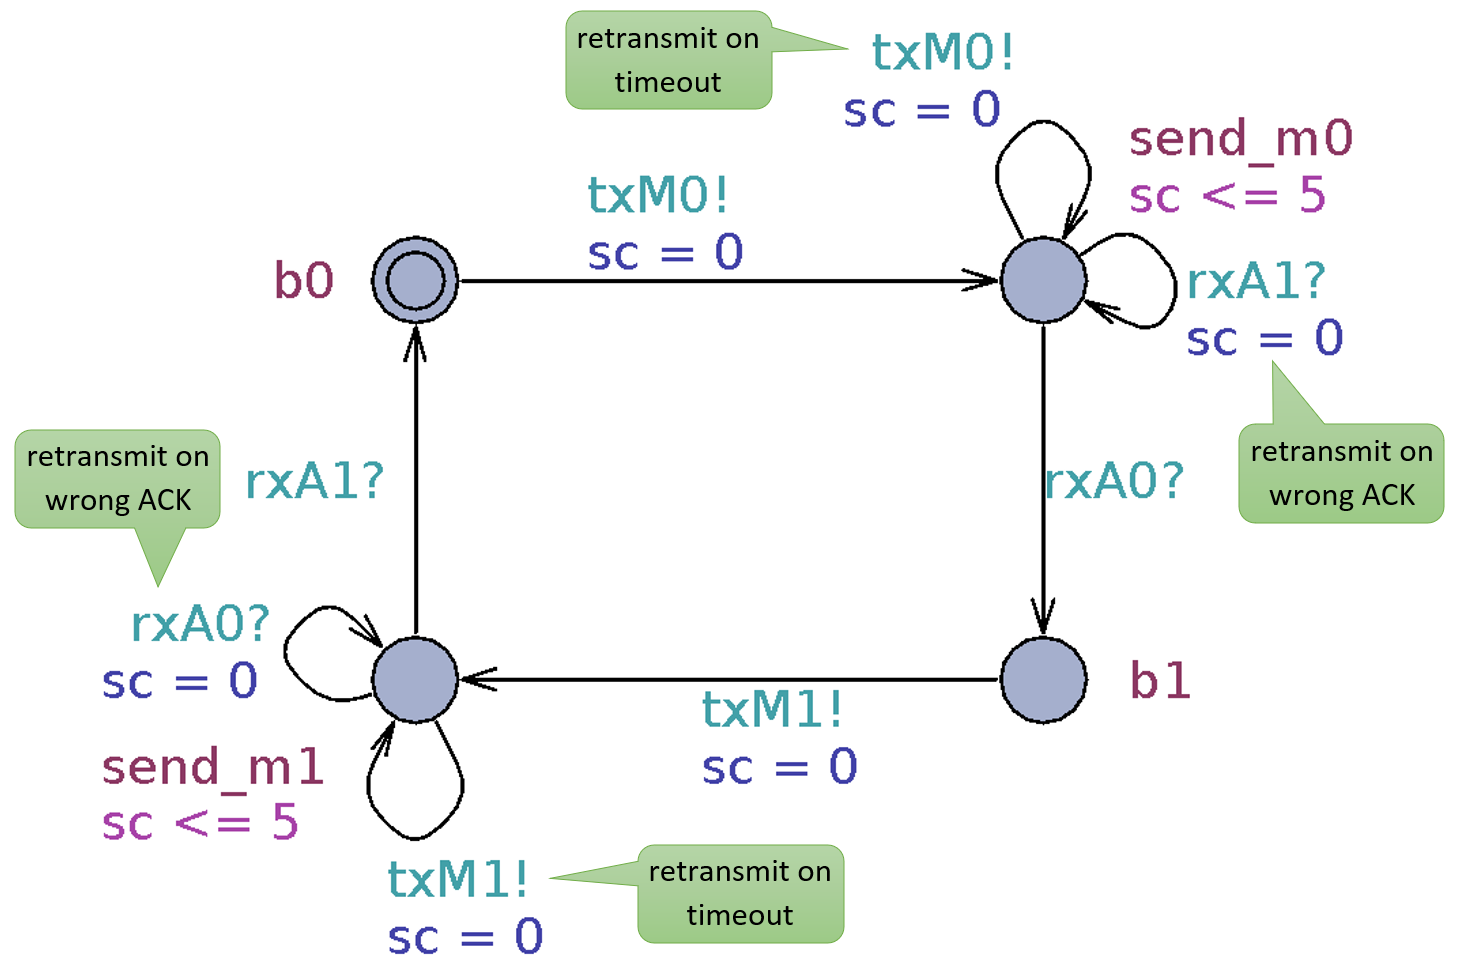
\includegraphics[width=38pc]{uppaal_tx.png}}
	\caption{Reliable ABP Sender modelled in UPPAAL}
	\label{fig:uppaal_tx}
\end{figure}

\subsection{Receiver}

The receiver in Fig. \ref{fig:uppaal_rx} starts in the state \texttt{rcv\_m0} where it waits for a message \texttt{M0}. Similarly to the sender, it will retransmit the acknowledgement \texttt{A1} until it receives \texttt{M0} from the channel. The message \texttt{M1} will be ignored in this state.

\begin{figure}[H]
	\centerline{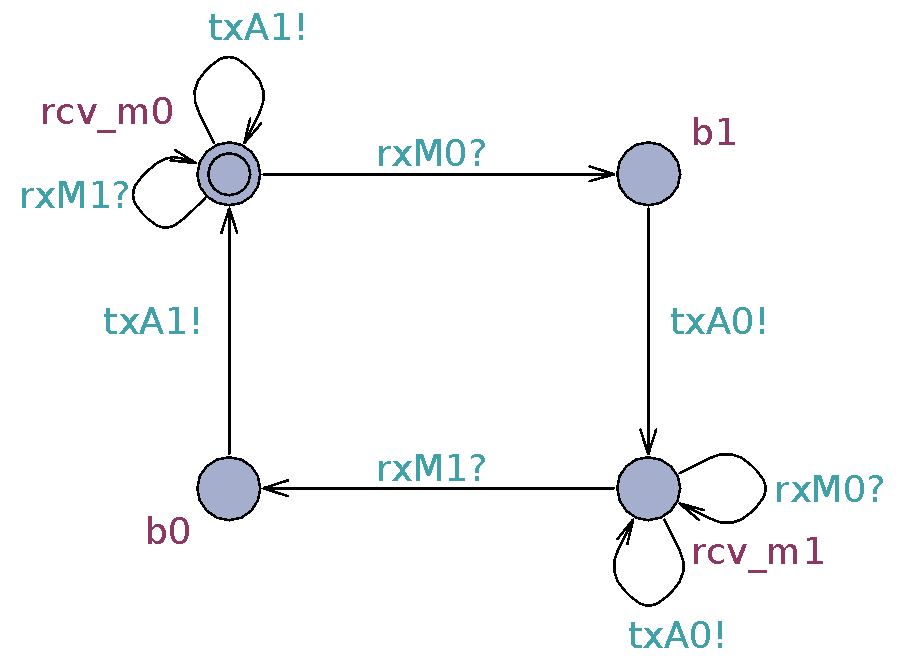
\includegraphics[width=28pc]{uppaal_rx.png}}
	\caption{ABP Receiver with ACK functionality modelled in UPPAAL}
	\label{fig:uppaal_rx}
\end{figure}

\subsection{Channel}

The channel in Fig. \ref{fig:uppaal_channel} takes the message transmissions from the sender and forwards them to the receiver and vice versa for the acknowledgment transmissions from the receiver.
There channel can however produce a bit flip (noise) or ignore a received packet entirely (loss).

\begin{figure}[H]
	\centerline{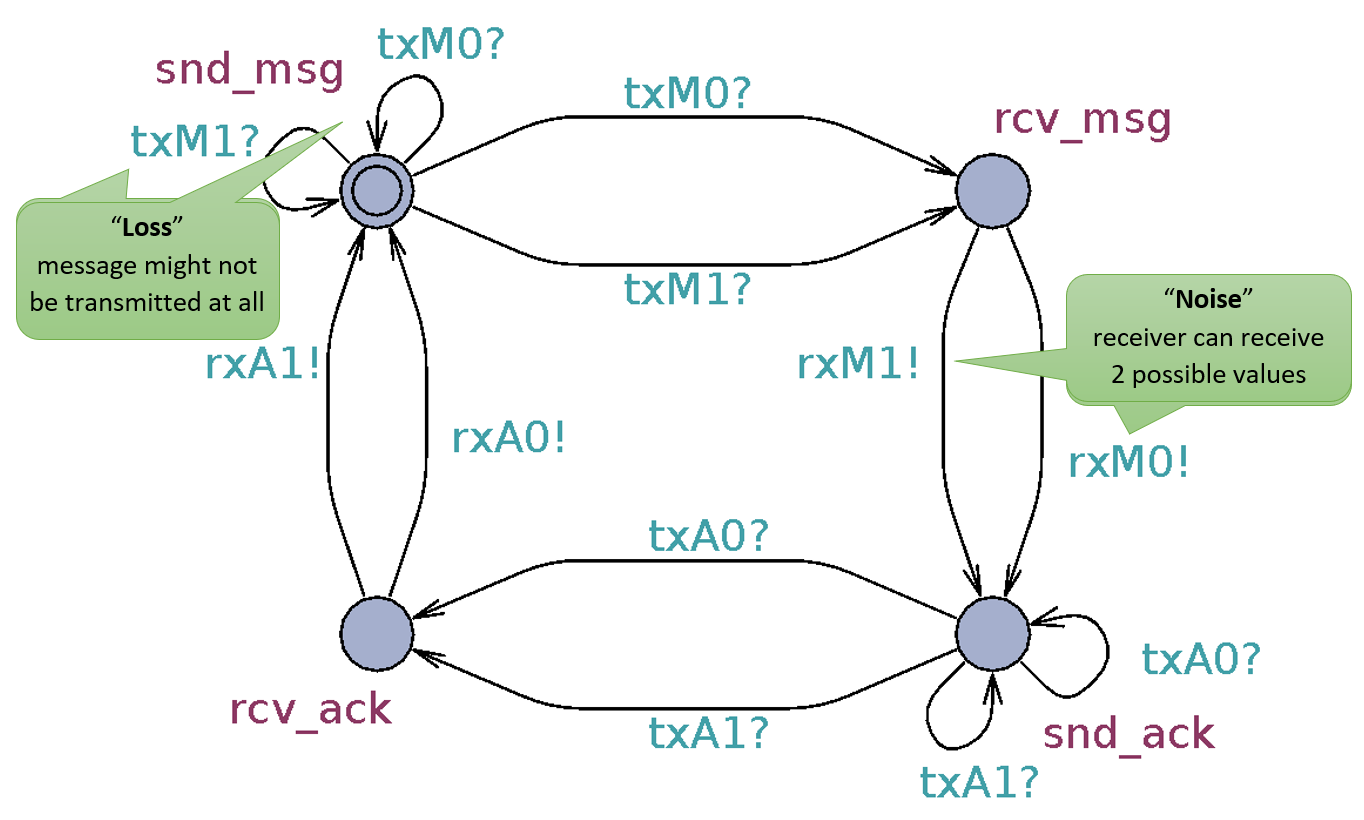
\includegraphics[width=38pc]{uppaal_channel.png}}
	\caption{Lossy and Noisy Channel for the ABP system}
	\label{fig:uppaal_channel}
\end{figure}

As visible in Fig. \ref{fig:uppaal_valid}, the system is deadlock free.
There exist the possibility for both the sender and the receiver to send, receive and acknowledge both the \texttt{0} and \texttt{1} messages.
However, the requirement that a message sent by the sender is eventually received by the receiver is not satisfied. This is entirely due to the non deterministic behavior of the channel. There is a chance that the channel contains so much noise or loss, that reliable transmission is not possible at all.
Or in other words, there exists a chance for $100$\% packet loss.

We can however make a probabilistic reasoning since there exist solutions where the messages are received correctly.
If we assume that the channel has a low loss rate and signal-to-noise ratio, communication can be performed reliably with the ABP.

\begin{figure}[H]
	\centerline{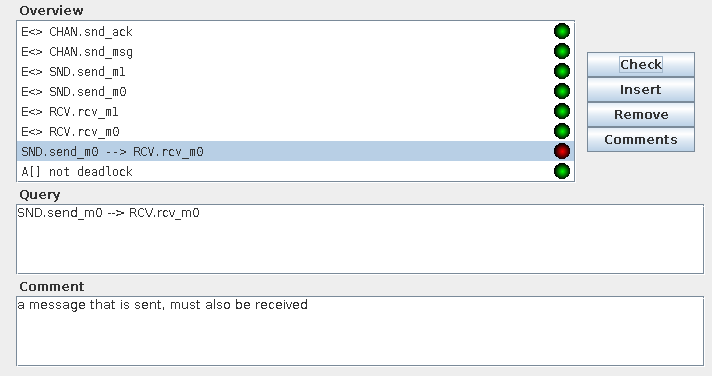
\includegraphics[width=30pc]{uppaal_valid.png}}
	\caption{Results of the system requirements}
	\label{fig:uppaal_valid}
\end{figure}

\end{document}
